\section{Synchronous events}\label{sec:syncev}

\SBGNERLone Version 2 allows the description of multiple consequences of the event that happens simultaneously. There are cases in which one interaction should influence several others in synchrony, for example the chemical reaction:

\begin{figure}[H]
  \centering
  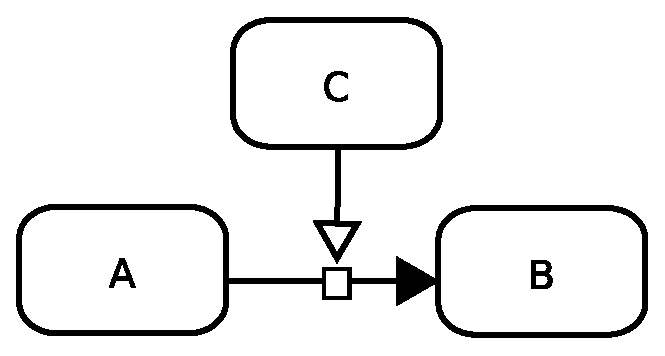
\includegraphics[scale = 0.75]{images/synchronous-PD}
  \caption{The reaction to represent in \ER.}
  \label{fig:synchronousPD}
\end{figure}

Having two outcomes and two stimulation links (\fig{asynchronous}) does not work in this case because all \corr{statement on}{statements of an} \ERm are independent. So it is possible that \glyph{entity} $B$ is created, but \glyph{entity} $A$ is not deleted. 

\begin{figure}[H]
  \centering
  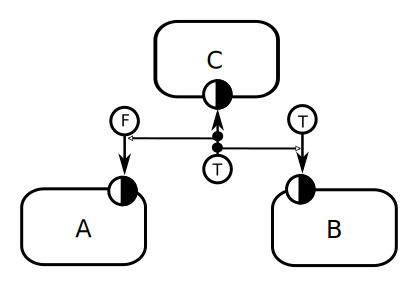
\includegraphics[scale = 0.75]{images/asynchronous}
  \caption{Independent events in \ER can not describe \fig{synchronousPD}.}
  \label{fig:asynchronous}
\end{figure}

To represent multiple consequences of the statement the influence arc is splitted \corr{to represent multiple consequences of the event}{} as shown in \fig{synchronous}. 

\begin{figure}[H]
  \centering
  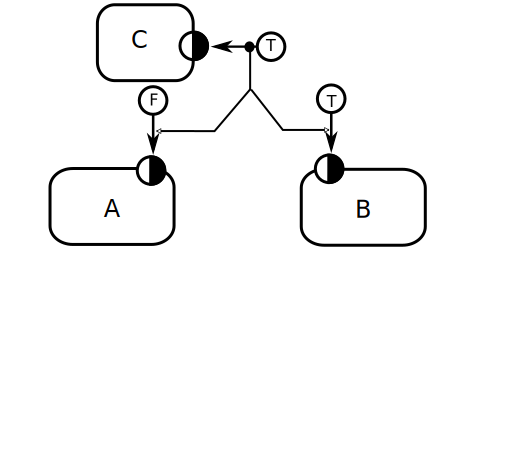
\includegraphics[scale = 0.75]{images/synchronous}
  \caption{The reaction from \fig{synchronousPD} in \ER.}
  \label{fig:synchronous}
\end{figure}

The diagram in \corr{the}{} \fig{synchronous} should be read as "If (or when) $C$ exists, it stimulates degradation of $A$ and creation of $B$ at the same time". 

Synchronous influences do not need to be of the same type and number of branches is not limited. A more general form of the proposed synchronous influence is presented in \fig{simultaneous}.

\begin{figure}[H]
  \centering
  \includegraphics[scale = 0.75]{images/simultaneous}
  \caption{Multiple synchronous consequences of the event.}
  \label{fig:simultaneous}
\end{figure}


Another example (\fig{gef}) is activation of small GTPase by Guanine nucleotide exchange factor (GEF).

\begin{figure}[H]
  \centering
  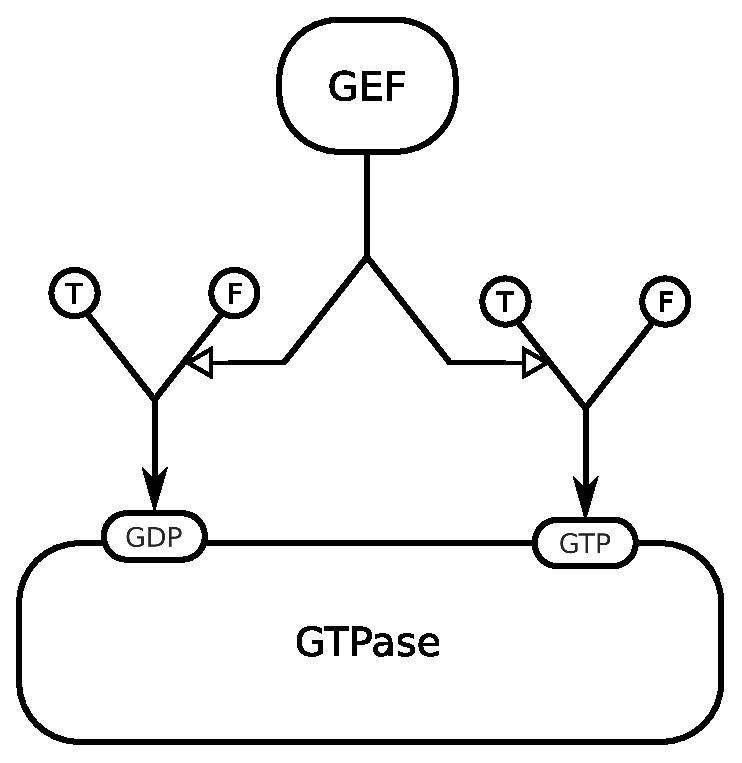
\includegraphics[scale = 0.75]{examples/gef}
  \caption{GTPase activation by GEF.}
  \label{fig:gef}
\end{figure}
